\documentclass[1p]{elsarticle_modified}
%\bibliographystyle{elsarticle-num}

%\usepackage[colorlinks]{hyperref}
%\usepackage{abbrmath_seonhwa} %\Abb, \Ascr, \Acal ,\Abf, \Afrak
\usepackage{amsfonts}
\usepackage{amssymb}
\usepackage{amsmath}
\usepackage{amsthm}
\usepackage{scalefnt}
\usepackage{amsbsy}
\usepackage{kotex}
\usepackage{caption}
\usepackage{subfig}
\usepackage{color}
\usepackage{graphicx}
\usepackage{xcolor} %% white, black, red, green, blue, cyan, magenta, yellow
\usepackage{float}
\usepackage{setspace}
\usepackage{hyperref}

\usepackage{tikz}
\usetikzlibrary{arrows}

\usepackage{multirow}
\usepackage{array} % fixed length table
\usepackage{hhline}

%%%%%%%%%%%%%%%%%%%%%
\makeatletter
\renewcommand*\env@matrix[1][\arraystretch]{%
	\edef\arraystretch{#1}%
	\hskip -\arraycolsep
	\let\@ifnextchar\new@ifnextchar
	\array{*\c@MaxMatrixCols c}}
\makeatother %https://tex.stackexchange.com/questions/14071/how-can-i-increase-the-line-spacing-in-a-matrix
%%%%%%%%%%%%%%%

\usepackage[normalem]{ulem}

\newcommand{\msout}[1]{\ifmmode\text{\sout{\ensuremath{#1}}}\else\sout{#1}\fi}
%SOURCE: \msout is \stkout macro in https://tex.stackexchange.com/questions/20609/strikeout-in-math-mode

\newcommand{\cancel}[1]{
	\ifmmode
	{\color{red}\msout{#1}}
	\else
	{\color{red}\sout{#1}}
	\fi
}

\newcommand{\add}[1]{
	{\color{blue}\uwave{#1}}
}

\newcommand{\replace}[2]{
	\ifmmode
	{\color{red}\msout{#1}}{\color{blue}\uwave{#2}}
	\else
	{\color{red}\sout{#1}}{\color{blue}\uwave{#2}}
	\fi
}

\newcommand{\Sol}{\mathcal{S}} %segment
\newcommand{\D}{D} %diagram
\newcommand{\A}{\mathcal{A}} %arc


%%%%%%%%%%%%%%%%%%%%%%%%%%%%%5 test

\def\sl{\operatorname{\textup{SL}}(2,\Cbb)}
\def\psl{\operatorname{\textup{PSL}}(2,\Cbb)}
\def\quan{\mkern 1mu \triangleright \mkern 1mu}

\theoremstyle{definition}
\newtheorem{thm}{Theorem}[section]
\newtheorem{prop}[thm]{Proposition}
\newtheorem{lem}[thm]{Lemma}
\newtheorem{ques}[thm]{Question}
\newtheorem{cor}[thm]{Corollary}
\newtheorem{defn}[thm]{Definition}
\newtheorem{exam}[thm]{Example}
\newtheorem{rmk}[thm]{Remark}
\newtheorem{alg}[thm]{Algorithm}

\newcommand{\I}{\sqrt{-1}}
\begin{document}

%\begin{frontmatter}
%
%\title{Boundary parabolic representations of knots up to 8 crossings}
%
%%% Group authors per affiliation:
%\author{Yunhi Cho} 
%\address{Department of Mathematics, University of Seoul, Seoul, Korea}
%\ead{yhcho@uos.ac.kr}
%
%
%\author{Seonhwa Kim} %\fnref{s_kim}}
%\address{Center for Geometry and Physics, Institute for Basic Science, Pohang, 37673, Korea}
%\ead{ryeona17@ibs.re.kr}
%
%\author{Hyuk Kim}
%\address{Department of Mathematical Sciences, Seoul National University, Seoul 08826, Korea}
%\ead{hyukkim@snu.ac.kr}
%
%\author{Seokbeom Yoon}
%\address{Department of Mathematical Sciences, Seoul National University, Seoul, 08826,  Korea}
%\ead{sbyoon15@snu.ac.kr}
%
%\begin{abstract}
%We find all boundary parabolic representation of knots up to 8 crossings.
%
%\end{abstract}
%\begin{keyword}
%    \MSC[2010] 57M25 
%\end{keyword}
%
%\end{frontmatter}

%\linenumbers
%\tableofcontents
%
\newcommand\colored[1]{\textcolor{white}{\rule[-0.35ex]{0.8em}{1.4ex}}\kern-0.8em\color{red} #1}%
%\newcommand\colored[1]{\textcolor{white}{ #1}\kern-2.17ex	\textcolor{white}{ #1}\kern-1.81ex	\textcolor{white}{ #1}\kern-2.15ex\color{red}#1	}

{\Large $\underline{12n_{0793}~(K12n_{0793})}$}

\setlength{\tabcolsep}{10pt}
\renewcommand{\arraystretch}{1.6}
\vspace{1cm}\begin{tabular}{m{100pt}>{\centering\arraybackslash}m{274pt}}
\multirow{5}{120pt}{
	\centering
	\includegraphics[width=112pt]{../../../GIT/diagram.site/Diagrams/png/2882_12n_0793.png}\\
\ \ \ A knot diagram\footnotemark}&
\allowdisplaybreaks
\textbf{Linearized knot diagam} \\
\cline{2-2}
 &
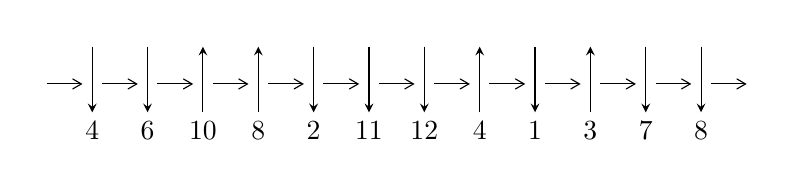
\begin{tikzpicture}[x=20pt, y=17pt]
	% nodes
	\node (C0) at (0, 0) {};
	\node (C1) at (1, 0) {};
	\node (C1U) at (1, +1) {};
	\node (C1D) at (1, -1) {4};

	\node (C2) at (2, 0) {};
	\node (C2U) at (2, +1) {};
	\node (C2D) at (2, -1) {6};

	\node (C3) at (3, 0) {};
	\node (C3U) at (3, +1) {};
	\node (C3D) at (3, -1) {10};

	\node (C4) at (4, 0) {};
	\node (C4U) at (4, +1) {};
	\node (C4D) at (4, -1) {8};

	\node (C5) at (5, 0) {};
	\node (C5U) at (5, +1) {};
	\node (C5D) at (5, -1) {2};

	\node (C6) at (6, 0) {};
	\node (C6U) at (6, +1) {};
	\node (C6D) at (6, -1) {11};

	\node (C7) at (7, 0) {};
	\node (C7U) at (7, +1) {};
	\node (C7D) at (7, -1) {12};

	\node (C8) at (8, 0) {};
	\node (C8U) at (8, +1) {};
	\node (C8D) at (8, -1) {4};

	\node (C9) at (9, 0) {};
	\node (C9U) at (9, +1) {};
	\node (C9D) at (9, -1) {1};

	\node (C10) at (10, 0) {};
	\node (C10U) at (10, +1) {};
	\node (C10D) at (10, -1) {3};

	\node (C11) at (11, 0) {};
	\node (C11U) at (11, +1) {};
	\node (C11D) at (11, -1) {7};

	\node (C12) at (12, 0) {};
	\node (C12U) at (12, +1) {};
	\node (C12D) at (12, -1) {8};
	\node (C13) at (13, 0) {};

	% arrows
	\draw[->,>={angle 60}]
	(C0) edge (C1) (C1) edge (C2) (C2) edge (C3) (C3) edge (C4) (C4) edge (C5) (C5) edge (C6) (C6) edge (C7) (C7) edge (C8) (C8) edge (C9) (C9) edge (C10) (C10) edge (C11) (C11) edge (C12) (C12) edge (C13) ;	\draw[->,>=stealth]
	(C1U) edge (C1D) (C2U) edge (C2D) (C3D) edge (C3U) (C4D) edge (C4U) (C5U) edge (C5D) (C6U) edge (C6D) (C7U) edge (C7D) (C8D) edge (C8U) (C9U) edge (C9D) (C10D) edge (C10U) (C11U) edge (C11D) (C12U) edge (C12D) ;
	\end{tikzpicture} \\
\hhline{~~} \\& 
\textbf{Solving Sequence} \\ \cline{2-2} 
 &
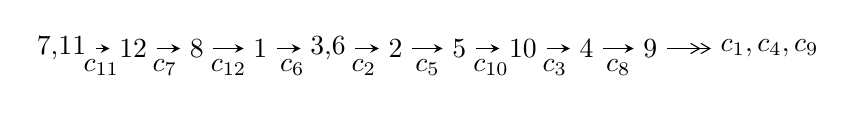
\begin{tikzpicture}[x=23pt, y=7pt]
	% node
	\node (A0) at (-1/8, 0) {7,11};
	\node (A1) at (1, 0) {12};
	\node (A2) at (2, 0) {8};
	\node (A3) at (3, 0) {1};
	\node (A4) at (65/16, 0) {3,6};
	\node (A5) at (41/8, 0) {2};
	\node (A6) at (49/8, 0) {5};
	\node (A7) at (57/8, 0) {10};
	\node (A8) at (65/8, 0) {4};
	\node (A9) at (73/8, 0) {9};
	\node (C1) at (1/2, -1) {$c_{11}$};
	\node (C2) at (3/2, -1) {$c_{7}$};
	\node (C3) at (5/2, -1) {$c_{12}$};
	\node (C4) at (7/2, -1) {$c_{6}$};
	\node (C5) at (37/8, -1) {$c_{2}$};
	\node (C6) at (45/8, -1) {$c_{5}$};
	\node (C7) at (53/8, -1) {$c_{10}$};
	\node (C8) at (61/8, -1) {$c_{3}$};
	\node (C9) at (69/8, -1) {$c_{8}$};
	\node (A10) at (11, 0) {$c_{1},c_{4},c_{9}$};

	% edge
	\draw[->,>=stealth]	
	(A0) edge (A1) (A1) edge (A2) (A2) edge (A3) (A3) edge (A4) (A4) edge (A5) (A5) edge (A6) (A6) edge (A7) (A7) edge (A8) (A8) edge (A9) ;
	\draw[->>,>={angle 60}]	
	(A9) edge (A10);
\end{tikzpicture} \\ 

\end{tabular} \\

\footnotetext{
The image of knot diagram is generated by the software ``\textbf{Draw programme}" developed by Andrew Bartholomew(\url{http://www.layer8.co.uk/maths/draw/index.htm\#Running-draw}), where we modified some parts for our purpose(\url{https://github.com/CATsTAILs/LinksPainter}).
}\phantom \\ \newline 
\centering \textbf{Ideals for irreducible components\footnotemark of $X_{\text{par}}$} 
 
\begin{align*}
I^u_{1}&=\langle 
-9.06380\times10^{25} u^{41}+1.37425\times10^{28} u^{40}+\cdots+2.41942\times10^{28} b-1.11983\times10^{29},\\
\phantom{I^u_{1}}&\phantom{= \langle  }-3.26749\times10^{28} u^{41}-3.64396\times10^{28} u^{40}+\cdots+2.66137\times10^{29} a+8.28132\times10^{29},\\
\phantom{I^u_{1}}&\phantom{= \langle  }u^{42}+2 u^{41}+\cdots-46 u+11\rangle \\
I^u_{2}&=\langle 
u^7-5 u^5+7 u^3+b-2 u,\;u^7-5 u^5+7 u^3- u^2+a-2 u+2,\\
\phantom{I^u_{2}}&\phantom{= \langle  }u^{12}+u^{11}-8 u^{10}-7 u^9+24 u^8+17 u^7-33 u^6-16 u^5+20 u^4+4 u^3-4 u^2- u-1\rangle \\
\\
\end{align*}
\raggedright * 2 irreducible components of $\dim_{\mathbb{C}}=0$, with total 54 representations.\\
\footnotetext{All coefficients of polynomials are rational numbers. But the coefficients are sometimes approximated in decimal forms when there is not enough margin.}
\newpage
\renewcommand{\arraystretch}{1}
\centering \section*{I. $I^u_{1}= \langle -9.06\times10^{25} u^{41}+1.37\times10^{28} u^{40}+\cdots+2.42\times10^{28} b-1.12\times10^{29},\;-3.27\times10^{28} u^{41}-3.64\times10^{28} u^{40}+\cdots+2.66\times10^{29} a+8.28\times10^{29},\;u^{42}+2 u^{41}+\cdots-46 u+11 \rangle$}
\flushleft \textbf{(i) Arc colorings}\\
\begin{tabular}{m{7pt} m{180pt} m{7pt} m{180pt} }
\flushright $a_{7}=$&$\begin{pmatrix}0\\u\end{pmatrix}$ \\
\flushright $a_{11}=$&$\begin{pmatrix}1\\0\end{pmatrix}$ \\
\flushright $a_{12}=$&$\begin{pmatrix}1\\u^2\end{pmatrix}$ \\
\flushright $a_{8}=$&$\begin{pmatrix}- u\\- u^3+u\end{pmatrix}$ \\
\flushright $a_{1}=$&$\begin{pmatrix}- u^2+1\\- u^4+2 u^2\end{pmatrix}$ \\
\flushright $a_{3}=$&$\begin{pmatrix}0.122775 u^{41}+0.136921 u^{40}+\cdots+9.26541 u-3.11168\\0.00374626 u^{41}-0.568007 u^{40}+\cdots-19.2584 u+4.62848\end{pmatrix}$ \\
\flushright $a_{6}=$&$\begin{pmatrix}u\\u\end{pmatrix}$ \\
\flushright $a_{2}=$&$\begin{pmatrix}0.552701 u^{41}+0.271165 u^{40}+\cdots-10.9013 u+2.02390\\0.433672 u^{41}-0.433763 u^{40}+\cdots-39.4251 u+9.76406\end{pmatrix}$ \\
\flushright $a_{5}=$&$\begin{pmatrix}1.16210 u^{41}+1.69216 u^{40}+\cdots+6.54468 u-3.34003\\0.919505 u^{41}+0.221580 u^{40}+\cdots-40.9514 u+10.5711\end{pmatrix}$ \\
\flushright $a_{10}=$&$\begin{pmatrix}1.17084 u^{41}+1.34160 u^{40}+\cdots-4.55540 u-2.12767\\1.14646 u^{41}+1.21035 u^{40}+\cdots-7.23546 u-2.71408\end{pmatrix}$ \\
\flushright $a_{4}=$&$\begin{pmatrix}0.785947 u^{41}+1.09699 u^{40}+\cdots+0.412589 u-1.16966\\0.634717 u^{41}+0.515957 u^{40}+\cdots-23.4534 u+6.67222\end{pmatrix}$ \\
\flushright $a_{9}=$&$\begin{pmatrix}-1.45613 u^{41}-1.65616 u^{40}+\cdots+6.43111 u+2.36059\\-1.31980 u^{41}-1.39650 u^{40}+\cdots+8.42549 u+3.12293\end{pmatrix}$\\&\end{tabular}
\flushleft \textbf{(ii) Obstruction class $= -1$}\\~\\
\flushleft \textbf{(iii) Cusp Shapes $= 0.0586366 u^{41}+0.331503 u^{40}+\cdots+5.71695 u-17.0612$}\\~\\
\newpage\renewcommand{\arraystretch}{1}
\flushleft \textbf{(iv) u-Polynomials at the component}\newline \\
\begin{tabular}{m{50pt}|m{274pt}}
Crossings & \hspace{64pt}u-Polynomials at each crossing \\
\hline $$\begin{aligned}c_{1}\end{aligned}$$&$\begin{aligned}
&u^{42}-2 u^{41}+\cdots-45 u-1
\end{aligned}$\\
\hline $$\begin{aligned}c_{2},c_{5}\end{aligned}$$&$\begin{aligned}
&u^{42}+3 u^{41}+\cdots+3244 u+611
\end{aligned}$\\
\hline $$\begin{aligned}c_{3},c_{10}\end{aligned}$$&$\begin{aligned}
&u^{42}+u^{41}+\cdots-26 u+7
\end{aligned}$\\
\hline $$\begin{aligned}c_{4},c_{8}\end{aligned}$$&$\begin{aligned}
&u^{42}-3 u^{41}+\cdots+222 u+79
\end{aligned}$\\
\hline $$\begin{aligned}c_{6},c_{7},c_{11}\\c_{12}\end{aligned}$$&$\begin{aligned}
&u^{42}-2 u^{41}+\cdots+46 u+11
\end{aligned}$\\
\hline $$\begin{aligned}c_{9}\end{aligned}$$&$\begin{aligned}
&u^{42}+u^{41}+\cdots-48 u+1
\end{aligned}$\\
\hline
\end{tabular}\\~\\
\newpage\renewcommand{\arraystretch}{1}
\flushleft \textbf{(v) Riley Polynomials at the component}\newline \\
\begin{tabular}{m{50pt}|m{274pt}}
Crossings & \hspace{64pt}Riley Polynomials at each crossing \\
\hline $$\begin{aligned}c_{1}\end{aligned}$$&$\begin{aligned}
&y^{42}+34 y^{41}+\cdots-3015 y+1
\end{aligned}$\\
\hline $$\begin{aligned}c_{2},c_{5}\end{aligned}$$&$\begin{aligned}
&y^{42}-29 y^{41}+\cdots-6104784 y+373321
\end{aligned}$\\
\hline $$\begin{aligned}c_{3},c_{10}\end{aligned}$$&$\begin{aligned}
&y^{42}+43 y^{41}+\cdots-1208 y+49
\end{aligned}$\\
\hline $$\begin{aligned}c_{4},c_{8}\end{aligned}$$&$\begin{aligned}
&y^{42}-37 y^{41}+\cdots-146770 y+6241
\end{aligned}$\\
\hline $$\begin{aligned}c_{6},c_{7},c_{11}\\c_{12}\end{aligned}$$&$\begin{aligned}
&y^{42}-52 y^{41}+\cdots-2050 y+121
\end{aligned}$\\
\hline $$\begin{aligned}c_{9}\end{aligned}$$&$\begin{aligned}
&y^{42}+39 y^{41}+\cdots-3522 y+1
\end{aligned}$\\
\hline
\end{tabular}\\~\\
\newpage\flushleft \textbf{(vi) Complex Volumes and Cusp Shapes}
$$\begin{array}{c|c|c}  
\text{Solutions to }I^u_{1}& \I (\text{vol} + \sqrt{-1}CS) & \text{Cusp shape}\\
 \hline 
\begin{aligned}
u &= \phantom{-}0.221678 + 0.929619 I \\
a &= \phantom{-}0.236802 + 0.144006 I \\
b &= \phantom{-}0.200628 + 1.379120 I\end{aligned}
 & -0.23479 + 3.42452 I & -7.25006 - 2.36788 I \\ \hline\begin{aligned}
u &= \phantom{-}0.221678 - 0.929619 I \\
a &= \phantom{-}0.236802 - 0.144006 I \\
b &= \phantom{-}0.200628 - 1.379120 I\end{aligned}
 & -0.23479 - 3.42452 I & -7.25006 + 2.36788 I \\ \hline\begin{aligned}
u &= \phantom{-}0.834678 + 0.726650 I \\
a &= \phantom{-}0.942471 + 1.038720 I \\
b &= -0.32235 + 1.47004 I\end{aligned}
 & -2.09585 - 8.88492 I & -8.23343 + 6.33839 I \\ \hline\begin{aligned}
u &= \phantom{-}0.834678 - 0.726650 I \\
a &= \phantom{-}0.942471 - 1.038720 I \\
b &= -0.32235 - 1.47004 I\end{aligned}
 & -2.09585 + 8.88492 I & -8.23343 - 6.33839 I \\ \hline\begin{aligned}
u &= \phantom{-}0.839481\phantom{ +0.000000I} \\
a &= -0.147245\phantom{ +0.000000I} \\
b &= \phantom{-}0.446812\phantom{ +0.000000I}\end{aligned}
 & -1.61731\phantom{ +0.000000I} & -3.83040\phantom{ +0.000000I} \\ \hline\begin{aligned}
u &= -0.649459 + 0.528735 I \\
a &= \phantom{-}0.425369 - 0.221209 I \\
b &= -0.883358 - 0.331381 I\end{aligned}
 & \phantom{-}3.71527 + 4.57178 I & -4.48983 - 6.21438 I \\ \hline\begin{aligned}
u &= -0.649459 - 0.528735 I \\
a &= \phantom{-}0.425369 + 0.221209 I \\
b &= -0.883358 + 0.331381 I\end{aligned}
 & \phantom{-}3.71527 - 4.57178 I & -4.48983 + 6.21438 I \\ \hline\begin{aligned}
u &= -1.205320 + 0.086480 I \\
a &= -0.45359 + 1.35560 I \\
b &= \phantom{-}0.093741 + 0.991733 I\end{aligned}
 & -4.64795 + 1.97026 I & -11.59090 - 3.85800 I \\ \hline\begin{aligned}
u &= -1.205320 - 0.086480 I \\
a &= -0.45359 - 1.35560 I \\
b &= \phantom{-}0.093741 - 0.991733 I\end{aligned}
 & -4.64795 - 1.97026 I & -11.59090 + 3.85800 I \\ \hline\begin{aligned}
u &= \phantom{-}0.550462 + 0.540915 I \\
a &= -1.409400 - 0.043470 I \\
b &= \phantom{-}0.125351 - 1.359680 I\end{aligned}
 & -6.87451 - 1.88626 I & -7.91284 + 3.72193 I\\
 \hline 
 \end{array}$$\newpage$$\begin{array}{c|c|c}  
\text{Solutions to }I^u_{1}& \I (\text{vol} + \sqrt{-1}CS) & \text{Cusp shape}\\
 \hline 
\begin{aligned}
u &= \phantom{-}0.550462 - 0.540915 I \\
a &= -1.409400 + 0.043470 I \\
b &= \phantom{-}0.125351 + 1.359680 I\end{aligned}
 & -6.87451 + 1.88626 I & -7.91284 - 3.72193 I \\ \hline\begin{aligned}
u &= -0.560203 + 0.440638 I \\
a &= \phantom{-}1.43565 - 1.00821 I \\
b &= -0.04993 - 1.58808 I\end{aligned}
 & -7.60002 + 1.56574 I & -5.17924 - 4.63604 I \\ \hline\begin{aligned}
u &= -0.560203 - 0.440638 I \\
a &= \phantom{-}1.43565 + 1.00821 I \\
b &= -0.04993 + 1.58808 I\end{aligned}
 & -7.60002 - 1.56574 I & -5.17924 + 4.63604 I \\ \hline\begin{aligned}
u &= -0.334964 + 0.627307 I \\
a &= -0.026307 + 1.176530 I \\
b &= \phantom{-}0.577071 - 0.144380 I\end{aligned}
 & \phantom{-}4.67940 - 0.63289 I & -1.299354 - 0.211342 I \\ \hline\begin{aligned}
u &= -0.334964 - 0.627307 I \\
a &= -0.026307 - 1.176530 I \\
b &= \phantom{-}0.577071 + 0.144380 I\end{aligned}
 & \phantom{-}4.67940 + 0.63289 I & -1.299354 + 0.211342 I \\ \hline\begin{aligned}
u &= -1.244160 + 0.465780 I \\
a &= -0.79090 + 1.18454 I \\
b &= -0.025737 + 1.302660 I\end{aligned}
 & -4.81553 + 1.49702 I & \phantom{-0.000000 } 0 \\ \hline\begin{aligned}
u &= -1.244160 - 0.465780 I \\
a &= -0.79090 - 1.18454 I \\
b &= -0.025737 - 1.302660 I\end{aligned}
 & -4.81553 - 1.49702 I & \phantom{-0.000000 } 0 \\ \hline\begin{aligned}
u &= \phantom{-}0.595320 + 0.215476 I \\
a &= \phantom{-}0.20407 - 3.29680 I \\
b &= \phantom{-}0.272977 - 1.203760 I\end{aligned}
 & \phantom{-}1.45303 - 2.42211 I & -8.67176 + 3.95905 I \\ \hline\begin{aligned}
u &= \phantom{-}0.595320 - 0.215476 I \\
a &= \phantom{-}0.20407 + 3.29680 I \\
b &= \phantom{-}0.272977 + 1.203760 I\end{aligned}
 & \phantom{-}1.45303 + 2.42211 I & -8.67176 - 3.95905 I \\ \hline\begin{aligned}
u &= \phantom{-}1.42044 + 0.21754 I \\
a &= -0.455901 + 0.764179 I \\
b &= -0.205009 + 0.109418 I\end{aligned}
 & -0.93890 - 2.37365 I & \phantom{-0.000000 } 0\\
 \hline 
 \end{array}$$\newpage$$\begin{array}{c|c|c}  
\text{Solutions to }I^u_{1}& \I (\text{vol} + \sqrt{-1}CS) & \text{Cusp shape}\\
 \hline 
\begin{aligned}
u &= \phantom{-}1.42044 - 0.21754 I \\
a &= -0.455901 - 0.764179 I \\
b &= -0.205009 - 0.109418 I\end{aligned}
 & -0.93890 + 2.37365 I & \phantom{-0.000000 } 0 \\ \hline\begin{aligned}
u &= \phantom{-}0.509507 + 0.231007 I \\
a &= \phantom{-}0.734692 - 0.787767 I \\
b &= -0.636452 - 1.034150 I\end{aligned}
 & \phantom{-}1.69283 + 0.80157 I & -9.60902 + 2.15996 I \\ \hline\begin{aligned}
u &= \phantom{-}0.509507 - 0.231007 I \\
a &= \phantom{-}0.734692 + 0.787767 I \\
b &= -0.636452 + 1.034150 I\end{aligned}
 & \phantom{-}1.69283 - 0.80157 I & -9.60902 - 2.15996 I \\ \hline\begin{aligned}
u &= -0.506114\phantom{ +0.000000I} \\
a &= -1.86988\phantom{ +0.000000I} \\
b &= \phantom{-}0.407424\phantom{ +0.000000I}\end{aligned}
 & -2.40722\phantom{ +0.000000I} & \phantom{-}5.24600\phantom{ +0.000000I} \\ \hline\begin{aligned}
u &= -1.56067 + 0.05190 I \\
a &= \phantom{-}0.204618 - 1.091020 I \\
b &= \phantom{-}0.907751 - 0.996705 I\end{aligned}
 & -5.42360 + 0.16996 I & \phantom{-0.000000 } 0 \\ \hline\begin{aligned}
u &= -1.56067 - 0.05190 I \\
a &= \phantom{-}0.204618 + 1.091020 I \\
b &= \phantom{-}0.907751 + 0.996705 I\end{aligned}
 & -5.42360 - 0.16996 I & \phantom{-0.000000 } 0 \\ \hline\begin{aligned}
u &= \phantom{-}1.56797\phantom{ +0.000000I} \\
a &= \phantom{-}0.157767\phantom{ +0.000000I} \\
b &= -0.854086\phantom{ +0.000000I}\end{aligned}
 & -9.60649\phantom{ +0.000000I} & \phantom{-0.000000 } 0 \\ \hline\begin{aligned}
u &= -1.58059 + 0.15570 I \\
a &= \phantom{-}0.76812 - 1.50303 I \\
b &= -0.36026 - 1.39238 I\end{aligned}
 & -14.1195 + 4.4084 I & \phantom{-0.000000 } 0 \\ \hline\begin{aligned}
u &= -1.58059 - 0.15570 I \\
a &= \phantom{-}0.76812 + 1.50303 I \\
b &= -0.36026 + 1.39238 I\end{aligned}
 & -14.1195 - 4.4084 I & \phantom{-0.000000 } 0 \\ \hline\begin{aligned}
u &= \phantom{-}1.58699 + 0.12206 I \\
a &= -0.62381 - 2.20399 I \\
b &= \phantom{-}0.15580 - 1.70095 I\end{aligned}
 & -14.9835 - 3.5968 I & \phantom{-0.000000 } 0\\
 \hline 
 \end{array}$$\newpage$$\begin{array}{c|c|c}  
\text{Solutions to }I^u_{1}& \I (\text{vol} + \sqrt{-1}CS) & \text{Cusp shape}\\
 \hline 
\begin{aligned}
u &= \phantom{-}1.58699 - 0.12206 I \\
a &= -0.62381 + 2.20399 I \\
b &= \phantom{-}0.15580 + 1.70095 I\end{aligned}
 & -14.9835 + 3.5968 I & \phantom{-0.000000 } 0 \\ \hline\begin{aligned}
u &= -1.59898 + 0.06331 I \\
a &= -0.27626 - 2.55653 I \\
b &= -0.08483 - 1.42792 I\end{aligned}
 & -6.19779 + 3.44957 I & \phantom{-0.000000 } 0 \\ \hline\begin{aligned}
u &= -1.59898 - 0.06331 I \\
a &= -0.27626 + 2.55653 I \\
b &= -0.08483 + 1.42792 I\end{aligned}
 & -6.19779 - 3.44957 I & \phantom{-0.000000 } 0 \\ \hline\begin{aligned}
u &= \phantom{-}1.59624 + 0.14855 I \\
a &= \phantom{-}0.294078 - 0.648191 I \\
b &= \phantom{-}1.115930 - 0.471602 I\end{aligned}
 & -3.89460 - 7.04306 I & \phantom{-0.000000 } 0 \\ \hline\begin{aligned}
u &= \phantom{-}1.59624 - 0.14855 I \\
a &= \phantom{-}0.294078 + 0.648191 I \\
b &= \phantom{-}1.115930 + 0.471602 I\end{aligned}
 & -3.89460 + 7.04306 I & \phantom{-0.000000 } 0 \\ \hline\begin{aligned}
u &= \phantom{-}0.230807 + 0.288001 I \\
a &= \phantom{-}0.966776 + 0.311482 I \\
b &= -0.188196 + 0.489488 I\end{aligned}
 & -0.234295 - 0.833962 I & -5.60412 + 8.29990 I \\ \hline\begin{aligned}
u &= \phantom{-}0.230807 - 0.288001 I \\
a &= \phantom{-}0.966776 - 0.311482 I \\
b &= -0.188196 - 0.489488 I\end{aligned}
 & -0.234295 + 0.833962 I & -5.60412 - 8.29990 I \\ \hline\begin{aligned}
u &= -1.66654 + 0.22609 I \\
a &= -0.61931 + 1.92291 I \\
b &= \phantom{-}0.40841 + 1.58400 I\end{aligned}
 & -10.5286 + 12.5719 I & \phantom{-0.000000 } 0 \\ \hline\begin{aligned}
u &= -1.66654 - 0.22609 I \\
a &= -0.61931 - 1.92291 I \\
b &= \phantom{-}0.40841 - 1.58400 I\end{aligned}
 & -10.5286 - 12.5719 I & \phantom{-0.000000 } 0 \\ \hline\begin{aligned}
u &= -1.69539\phantom{ +0.000000I} \\
a &= -0.0379052\phantom{ +0.000000I} \\
b &= -0.681558\phantom{ +0.000000I}\end{aligned}
 & -10.7530\phantom{ +0.000000I} & \phantom{-0.000000 } 0\\
 \hline 
 \end{array}$$\newpage$$\begin{array}{c|c|c}  
\text{Solutions to }I^u_{1}& \I (\text{vol} + \sqrt{-1}CS) & \text{Cusp shape}\\
 \hline 
\begin{aligned}
u &= \phantom{-}1.75180 + 0.08364 I \\
a &= \phantom{-}0.43693 + 1.85011 I \\
b &= -0.26084 + 1.40596 I\end{aligned}
 & -15.4551 - 3.4434 I & \phantom{-0.000000 } 0 \\ \hline\begin{aligned}
u &= \phantom{-}1.75180 - 0.08364 I \\
a &= \phantom{-}0.43693 - 1.85011 I \\
b &= -0.26084 - 1.40596 I\end{aligned}
 & -15.4551 + 3.4434 I & \phantom{-0.000000 } 0\\
 \hline 
 \end{array}$$\newpage\newpage\renewcommand{\arraystretch}{1}
\centering \section*{II. $I^u_{2}= \langle u^7-5 u^5+7 u^3+b-2 u,\;u^7-5 u^5+7 u^3- u^2+a-2 u+2,\;u^{12}+u^{11}+\cdots- u-1 \rangle$}
\flushleft \textbf{(i) Arc colorings}\\
\begin{tabular}{m{7pt} m{180pt} m{7pt} m{180pt} }
\flushright $a_{7}=$&$\begin{pmatrix}0\\u\end{pmatrix}$ \\
\flushright $a_{11}=$&$\begin{pmatrix}1\\0\end{pmatrix}$ \\
\flushright $a_{12}=$&$\begin{pmatrix}1\\u^2\end{pmatrix}$ \\
\flushright $a_{8}=$&$\begin{pmatrix}- u\\- u^3+u\end{pmatrix}$ \\
\flushright $a_{1}=$&$\begin{pmatrix}- u^2+1\\- u^4+2 u^2\end{pmatrix}$ \\
\flushright $a_{3}=$&$\begin{pmatrix}- u^7+5 u^5-7 u^3+u^2+2 u-2\\- u^7+5 u^5-7 u^3+2 u\end{pmatrix}$ \\
\flushright $a_{6}=$&$\begin{pmatrix}u\\u\end{pmatrix}$ \\
\flushright $a_{2}=$&$\begin{pmatrix}- u^7+5 u^5- u^4-7 u^3+3 u^2+2 u-2\\- u^7+5 u^5- u^4-7 u^3+2 u^2+2 u\end{pmatrix}$ \\
\flushright $a_{5}=$&$\begin{pmatrix}- u^{10}+7 u^8- u^7-17 u^6+5 u^5+16 u^4-8 u^3-4 u^2+5 u\\- u^{10}+7 u^8- u^7-17 u^6+4 u^5+16 u^4-4 u^3-4 u^2+u\end{pmatrix}$ \\
\flushright $a_{10}=$&$\begin{pmatrix}- u^9+7 u^7-17 u^5+17 u^3-6 u\\u^3-2 u-1\end{pmatrix}$ \\
\flushright $a_{4}=$&$\begin{pmatrix}- u^{10}+7 u^8- u^7-17 u^6+6 u^5+16 u^4-11 u^3-4 u^2+6 u\\- u^{10}+7 u^8-17 u^6+16 u^4-4 u^2\end{pmatrix}$ \\
\flushright $a_{9}=$&$\begin{pmatrix}u^{11}-9 u^9+30 u^7-45 u^5+30 u^3-9 u-1\\- u-1\end{pmatrix}$\\&\end{tabular}
\flushleft \textbf{(ii) Obstruction class $= 1$}\\~\\
\flushleft \textbf{(iii) Cusp Shapes $= - u^{11}+6 u^9+u^8-10 u^7-10 u^6- u^5+29 u^4+10 u^3-27 u^2+u-7$}\\~\\
\newpage\renewcommand{\arraystretch}{1}
\flushleft \textbf{(iv) u-Polynomials at the component}\newline \\
\begin{tabular}{m{50pt}|m{274pt}}
Crossings & \hspace{64pt}u-Polynomials at each crossing \\
\hline $$\begin{aligned}c_{1}\end{aligned}$$&$\begin{aligned}
&u^{12}- u^{11}+3 u^{10}+u^8+3 u^7-2 u^6- u^5- u^4-4 u^3- u^2+2 u+1
\end{aligned}$\\
\hline $$\begin{aligned}c_{2}\end{aligned}$$&$\begin{aligned}
&u^{12}+2 u^{11}- u^{10}-4 u^9- u^8- u^7-2 u^6+3 u^5+u^4+3 u^2- u+1
\end{aligned}$\\
\hline $$\begin{aligned}c_{3}\end{aligned}$$&$\begin{aligned}
&u^{12}+7 u^{10}+19 u^8- u^7+25 u^6-4 u^5+16 u^4-5 u^3+3 u^2-3 u-1
\end{aligned}$\\
\hline $$\begin{aligned}c_{4}\end{aligned}$$&$\begin{aligned}
&u^{12}-2 u^{11}- u^{10}+4 u^9-3 u^8+4 u^7-7 u^5+4 u^4-7 u^3+8 u^2+3 u-1
\end{aligned}$\\
\hline $$\begin{aligned}c_{5}\end{aligned}$$&$\begin{aligned}
&u^{12}-2 u^{11}- u^{10}+4 u^9- u^8+u^7-2 u^6-3 u^5+u^4+3 u^2+u+1
\end{aligned}$\\
\hline $$\begin{aligned}c_{6},c_{7}\end{aligned}$$&$\begin{aligned}
&u^{12}- u^{11}+\cdots+u-1
\end{aligned}$\\
\hline $$\begin{aligned}c_{8}\end{aligned}$$&$\begin{aligned}
&u^{12}+2 u^{11}- u^{10}-4 u^9-3 u^8-4 u^7+7 u^5+4 u^4+7 u^3+8 u^2-3 u-1
\end{aligned}$\\
\hline $$\begin{aligned}c_{9}\end{aligned}$$&$\begin{aligned}
&u^{12}+3 u^{10}- u^9-2 u^7-8 u^6+7 u^5-4 u^4+15 u^3+4 u^2+u-3
\end{aligned}$\\
\hline $$\begin{aligned}c_{10}\end{aligned}$$&$\begin{aligned}
&u^{12}+7 u^{10}+19 u^8+u^7+25 u^6+4 u^5+16 u^4+5 u^3+3 u^2+3 u-1
\end{aligned}$\\
\hline $$\begin{aligned}c_{11},c_{12}\end{aligned}$$&$\begin{aligned}
&u^{12}+u^{11}+\cdots- u-1
\end{aligned}$\\
\hline
\end{tabular}\\~\\
\newpage\renewcommand{\arraystretch}{1}
\flushleft \textbf{(v) Riley Polynomials at the component}\newline \\
\begin{tabular}{m{50pt}|m{274pt}}
Crossings & \hspace{64pt}Riley Polynomials at each crossing \\
\hline $$\begin{aligned}c_{1}\end{aligned}$$&$\begin{aligned}
&y^{12}+5 y^{11}+\cdots-6 y+1
\end{aligned}$\\
\hline $$\begin{aligned}c_{2},c_{5}\end{aligned}$$&$\begin{aligned}
&y^{12}-6 y^{11}+\cdots+5 y+1
\end{aligned}$\\
\hline $$\begin{aligned}c_{3},c_{10}\end{aligned}$$&$\begin{aligned}
&y^{12}+14 y^{11}+\cdots-15 y+1
\end{aligned}$\\
\hline $$\begin{aligned}c_{4},c_{8}\end{aligned}$$&$\begin{aligned}
&y^{12}-6 y^{11}+\cdots-25 y+1
\end{aligned}$\\
\hline $$\begin{aligned}c_{6},c_{7},c_{11}\\c_{12}\end{aligned}$$&$\begin{aligned}
&y^{12}-17 y^{11}+\cdots+7 y+1
\end{aligned}$\\
\hline $$\begin{aligned}c_{9}\end{aligned}$$&$\begin{aligned}
&y^{12}+6 y^{11}+\cdots-25 y+9
\end{aligned}$\\
\hline
\end{tabular}\\~\\
\newpage\flushleft \textbf{(vi) Complex Volumes and Cusp Shapes}
$$\begin{array}{c|c|c}  
\text{Solutions to }I^u_{2}& \I (\text{vol} + \sqrt{-1}CS) & \text{Cusp shape}\\
 \hline 
\begin{aligned}
u &= \phantom{-}0.686882 + 0.356361 I \\
a &= -1.57192 - 1.03304 I \\
b &= \phantom{-}0.08327 - 1.52260 I\end{aligned}
 & -8.42506 - 1.23513 I & -14.9695 + 0.5232 I \\ \hline\begin{aligned}
u &= \phantom{-}0.686882 - 0.356361 I \\
a &= -1.57192 + 1.03304 I \\
b &= \phantom{-}0.08327 + 1.52260 I\end{aligned}
 & -8.42506 + 1.23513 I & -14.9695 - 0.5232 I \\ \hline\begin{aligned}
u &= -0.697854\phantom{ +0.000000I} \\
a &= -1.27667\phantom{ +0.000000I} \\
b &= \phantom{-}0.236332\phantom{ +0.000000I}\end{aligned}
 & -2.77397\phantom{ +0.000000I} & -17.7110\phantom{ +0.000000I} \\ \hline\begin{aligned}
u &= -1.350010 + 0.165727 I \\
a &= \phantom{-}0.122773 + 0.422338 I \\
b &= \phantom{-}0.327726 + 0.869804 I\end{aligned}
 & -1.87314 + 3.35889 I & -9.63200 - 3.88261 I \\ \hline\begin{aligned}
u &= -1.350010 - 0.165727 I \\
a &= \phantom{-}0.122773 - 0.422338 I \\
b &= \phantom{-}0.327726 - 0.869804 I\end{aligned}
 & -1.87314 - 3.35889 I & -9.63200 + 3.88261 I \\ \hline\begin{aligned}
u &= \phantom{-}1.43456 + 0.19655 I \\
a &= \phantom{-}0.38745 + 1.66784 I \\
b &= \phantom{-}0.368130 + 1.103920 I\end{aligned}
 & -2.74104 - 0.62345 I & -7.00640 - 0.32990 I \\ \hline\begin{aligned}
u &= \phantom{-}1.43456 - 0.19655 I \\
a &= \phantom{-}0.38745 - 1.66784 I \\
b &= \phantom{-}0.368130 - 1.103920 I\end{aligned}
 & -2.74104 + 0.62345 I & -7.00640 + 0.32990 I \\ \hline\begin{aligned}
u &= -0.076876 + 0.352057 I \\
a &= -2.49621 + 0.92625 I \\
b &= -0.378175 + 0.980375 I\end{aligned}
 & \phantom{-}2.45499 - 1.46473 I & -3.28668 + 1.82890 I \\ \hline\begin{aligned}
u &= -0.076876 - 0.352057 I \\
a &= -2.49621 - 0.92625 I \\
b &= -0.378175 - 0.980375 I\end{aligned}
 & \phantom{-}2.45499 + 1.46473 I & -3.28668 - 1.82890 I \\ \hline\begin{aligned}
u &= \phantom{-}1.67252\phantom{ +0.000000I} \\
a &= \phantom{-}0.219784\phantom{ +0.000000I} \\
b &= -0.577555\phantom{ +0.000000I}\end{aligned}
 & -11.3408\phantom{ +0.000000I} & -16.0060\phantom{ +0.000000I}\\
 \hline 
 \end{array}$$\newpage$$\begin{array}{c|c|c}  
\text{Solutions to }I^u_{2}& \I (\text{vol} + \sqrt{-1}CS) & \text{Cusp shape}\\
 \hline 
\begin{aligned}
u &= -1.68189 + 0.10991 I \\
a &= \phantom{-}0.58634 - 1.91439 I \\
b &= -0.23034 - 1.54467 I\end{aligned}
 & -16.9020 + 3.1092 I & -14.7470 - 0.9268 I \\ \hline\begin{aligned}
u &= -1.68189 - 0.10991 I \\
a &= \phantom{-}0.58634 + 1.91439 I \\
b &= -0.23034 + 1.54467 I\end{aligned}
 & -16.9020 - 3.1092 I & -14.7470 + 0.9268 I\\
 \hline 
 \end{array}$$\newpage
\newpage\renewcommand{\arraystretch}{1}
\centering \section*{ III. u-Polynomials}
\begin{tabular}{m{50pt}|m{274pt}}
Crossings & \hspace{64pt}u-Polynomials at each crossing \\
\hline $$\begin{aligned}c_{1}\end{aligned}$$&$\begin{aligned}
&(u^{12}- u^{11}+3 u^{10}+u^8+3 u^7-2 u^6- u^5- u^4-4 u^3- u^2+2 u+1)\\
&\cdot(u^{42}-2 u^{41}+\cdots-45 u-1)
\end{aligned}$\\
\hline $$\begin{aligned}c_{2}\end{aligned}$$&$\begin{aligned}
&(u^{12}+2 u^{11}- u^{10}-4 u^9- u^8- u^7-2 u^6+3 u^5+u^4+3 u^2- u+1)\\
&\cdot(u^{42}+3 u^{41}+\cdots+3244 u+611)
\end{aligned}$\\
\hline $$\begin{aligned}c_{3}\end{aligned}$$&$\begin{aligned}
&(u^{12}+7 u^{10}+19 u^8- u^7+25 u^6-4 u^5+16 u^4-5 u^3+3 u^2-3 u-1)\\
&\cdot(u^{42}+u^{41}+\cdots-26 u+7)
\end{aligned}$\\
\hline $$\begin{aligned}c_{4}\end{aligned}$$&$\begin{aligned}
&(u^{12}-2 u^{11}- u^{10}+4 u^9-3 u^8+4 u^7-7 u^5+4 u^4-7 u^3+8 u^2+3 u-1)\\
&\cdot(u^{42}-3 u^{41}+\cdots+222 u+79)
\end{aligned}$\\
\hline $$\begin{aligned}c_{5}\end{aligned}$$&$\begin{aligned}
&(u^{12}-2 u^{11}- u^{10}+4 u^9- u^8+u^7-2 u^6-3 u^5+u^4+3 u^2+u+1)\\
&\cdot(u^{42}+3 u^{41}+\cdots+3244 u+611)
\end{aligned}$\\
\hline $$\begin{aligned}c_{6},c_{7}\end{aligned}$$&$\begin{aligned}
&(u^{12}- u^{11}+\cdots+u-1)(u^{42}-2 u^{41}+\cdots+46 u+11)
\end{aligned}$\\
\hline $$\begin{aligned}c_{8}\end{aligned}$$&$\begin{aligned}
&(u^{12}+2 u^{11}- u^{10}-4 u^9-3 u^8-4 u^7+7 u^5+4 u^4+7 u^3+8 u^2-3 u-1)\\
&\cdot(u^{42}-3 u^{41}+\cdots+222 u+79)
\end{aligned}$\\
\hline $$\begin{aligned}c_{9}\end{aligned}$$&$\begin{aligned}
&(u^{12}+3 u^{10}- u^9-2 u^7-8 u^6+7 u^5-4 u^4+15 u^3+4 u^2+u-3)\\
&\cdot(u^{42}+u^{41}+\cdots-48 u+1)
\end{aligned}$\\
\hline $$\begin{aligned}c_{10}\end{aligned}$$&$\begin{aligned}
&(u^{12}+7 u^{10}+19 u^8+u^7+25 u^6+4 u^5+16 u^4+5 u^3+3 u^2+3 u-1)\\
&\cdot(u^{42}+u^{41}+\cdots-26 u+7)
\end{aligned}$\\
\hline $$\begin{aligned}c_{11},c_{12}\end{aligned}$$&$\begin{aligned}
&(u^{12}+u^{11}+\cdots- u-1)(u^{42}-2 u^{41}+\cdots+46 u+11)
\end{aligned}$\\
\hline
\end{tabular}\newpage\renewcommand{\arraystretch}{1}
\centering \section*{ IV. Riley Polynomials}
\begin{tabular}{m{50pt}|m{274pt}}
Crossings & \hspace{64pt}Riley Polynomials at each crossing \\
\hline $$\begin{aligned}c_{1}\end{aligned}$$&$\begin{aligned}
&(y^{12}+5 y^{11}+\cdots-6 y+1)(y^{42}+34 y^{41}+\cdots-3015 y+1)
\end{aligned}$\\
\hline $$\begin{aligned}c_{2},c_{5}\end{aligned}$$&$\begin{aligned}
&(y^{12}-6 y^{11}+\cdots+5 y+1)(y^{42}-29 y^{41}+\cdots-6104784 y+373321)
\end{aligned}$\\
\hline $$\begin{aligned}c_{3},c_{10}\end{aligned}$$&$\begin{aligned}
&(y^{12}+14 y^{11}+\cdots-15 y+1)(y^{42}+43 y^{41}+\cdots-1208 y+49)
\end{aligned}$\\
\hline $$\begin{aligned}c_{4},c_{8}\end{aligned}$$&$\begin{aligned}
&(y^{12}-6 y^{11}+\cdots-25 y+1)(y^{42}-37 y^{41}+\cdots-146770 y+6241)
\end{aligned}$\\
\hline $$\begin{aligned}c_{6},c_{7},c_{11}\\c_{12}\end{aligned}$$&$\begin{aligned}
&(y^{12}-17 y^{11}+\cdots+7 y+1)(y^{42}-52 y^{41}+\cdots-2050 y+121)
\end{aligned}$\\
\hline $$\begin{aligned}c_{9}\end{aligned}$$&$\begin{aligned}
&(y^{12}+6 y^{11}+\cdots-25 y+9)(y^{42}+39 y^{41}+\cdots-3522 y+1)
\end{aligned}$\\
\hline
\end{tabular}
\vskip 2pc
\end{document}